% Chapter Template

\chapter{Análisis y Diseño del Sistema} % Main chapter title

\label{Chapter4} % Change X to a consecutive number; for referencing this chapter elsewhere, use \ref{ChapterX}

\lhead{Capítulo 4. \emph{Análisis y Diseño del Sistema}} % Change X to a consecutive number; this is for the header on each page - perhaps a shortened title

%----------------------------------------------------------------------------------------
%	SECTION 1
%----------------------------------------------------------------------------------------
\setstretch{1.1} % Line spacing of 1.1
Luego de haber adquirido una amplia cantidad de conocimiento sobre la tecnología Blockchain en general y sobre Hyperledger Fabric en particular, el presente capítulo investiga los problemas que tiene la UNC con la gestión y validación de información académica. Para eso se realizó una entrevista con el Ingeniero Miguel Montes, Prosecretario de Informática de la UNC. Luego se procede a analizar si las soluciones propuestas a las cuales se llegaron en la entrevista representan un caso de uso de Blockchain. Por último, se especifican Componentes, Requerimientos y Comportamiento del sistema a implementar.

\section{Entrevista}
La entrevista fue conducida con el objetivo de validar las primeras especificaciones para el prototipo planteado en la sección \ref{sec:primeras_especificaciones_prototipo} y para lograr una perspicacia mejor de los problemas del sistema de gestión de alumnos Guaraní que podrían ser resueltos a través de un Blockchain.
Con respecto al sistema Guaraní, el Prosecretario Ing. Montes planteó los problemas siguientes:

\begin{itemize}
\item El primer problema es un problema de digitalización: Las actas actualmente se imprimen y se firman en papel por los profesores autorizados, luego es necesario almacenarlas. Se podría implementar un equivalente digital que se firma digitalmente. Eso presenta el problema de la firma en sí: Cada profesor debe tener su clave, por ejemplo en forma de un token de hardware, lo cual involucra varios problemas: En primer lugar, significa un alto costo de adquisición y luego se requiere administrar dicho recurso, ya que en el caso de daño o de pérdida, el token tiene que ser reemplazado. A su vez, no debe ser posible aceptar firmas realizadas con el token anterior, es decir, se debe mantener una lista negra para claves extraviadas. Además, los profesores deben ser capacitados para poder realizar las firmas correctamente. 

\item El segundo problema afecta la integridad y la disponibilidad de las actas: Actualmente, en el momento de un examen, el profesor es el responsable de otorgar una nota correspondiente al desempeño del alumno. Eso queda asentado, ya que ambos, alumnos como docentes, firman el acta. Sin embargo, no existe la misma responsabilidad en el caso del administrador de la base de datos: El encargado de subir la nota a la base de datos del sistema Guaraní podría modificar la información sin levantar sospecha. Un acta digitalmente firmada no podría modificarse sin que la firma pierda su validez, pero si un acta tiene un error y es rectificado, permanece con una firma válida. Acá es donde aparece el problema de disponibilidad: Frente a la desaparición del acta rectificadora, queda el acta rectificada con una firma válida y no sería posible detectar si el acta fue rectificada o no. 

\item En el caso del tercer problema se trata de interoperabilidad: Al principio, la adopción puede ser difícil, ya que todas las entidades que trabajan con los documentos en cuestión, tienen que cambiar a un sistema digital. Y si la distribución de dichos documentos se hiciera a través de un Blockchain, se originaría un problema legal - la información que se genera entre Universidad y alumno por ley no puede ser difundida a terceros.
\end{itemize}

Las soluciones propuestas en la entrevista fueron los siguientes: 
\begin{itemize}
\item Una de las propiedades características del Blockchain es su carácter inmutable cuando es lo suficientemente distribuido y bajo de control de una multitud de organismos. En el caso de utilizar Blockchain, los ataques contra la integridad y disponibilidad de las actas descritas anteriormente no serían posibles, ya que quedaría un registro inmutable de todas las actas y las actas rectificadoras.
\item Para resolver el problema de la privacidad de la información, se podría aplicar una función \textit{hash} a los datos en cuestión. Así, el Blockchain no sería un mecanismo de distribución de información, pero se podrían implementar \textit{smart contracts}, que validen certificados otorgados contra el Blockchain.
\item Siempre y cuando los demás organismos acepten los certificados emitidos y sean capaces de validarlos contra el Blockchain, se resuelve el problema de interoperabilidad. El usuario, que en este caso es el alumno, mantiene control sobre sus datos: él es responsable de presentar lo que corresponda ante el organismo en cuestión, y dicho organismo puede verificar la validez de lo presentado inmediatamente a través del Blockchain, sin embargo, sin los datos originales, no tiene acceso a ningún tipo de información privada.
\item El problema de la digitalización tiene que ser resuelto por cada facultad: Una opción propuesta por Montes consta de firmar las actas en papel en el momento del examen, para que luego sean escaneadas por una persona dedicada que certifica con una firma digital que las notas del acta original coinciden con las notas del acta digital. Un \textit{hash} del acta completo se agregaría al Blockchain. De este modo, la facultad evita la compra de una gran cantidad de tokens, ya que se requiere uno solo para la persona que escanea las actas. Además, se evita cambiar el modo de trabajo de muchos profesores a la hora de evaluar un examen.
\end{itemize}

\section{Casos de uso de Blockchain}
Desde el éxito de Bitcoin y el nacimiento de numerosas otras criptomonedas y plataformas Blockchain, existe mucha especulación sobre el impacto que va a tener la tecnología una vez que esté madura y adoptada. Para nombrar solo un ejemplo, \textit{The Economist} publicó una edición el 31 de octubre de 2015 en cuya portada figuraba el título ``La máquina de la confianza - cómo la tecnología detrás de Bitcoin podría cambiar al mundo.'' Gideon Greenspan, Fundador de la plataforma Multichain, describe el 22 de Noviembre del mismo año en un artículo con el nombre ``Evitar el proyecto Blockchain inútil'' que ``Estamos viendo un número cada vez mayor de compañías que crean pruebas de concepto en nuestra plataforma y / o piden nuestra ayuda.''

Para aclarar la confusión insiste en que no todos los casos de uso son adecuados para Blockchain: ``Si los requisitos se cumplen con usar las bases de datos relacionales de hoy, estarías loco si usas un Blockchain.'' Con el argumento que bases de datos relacionales tienen décadas de desarrollo y soportan miles de consultas por segundo, explica una serie de criterios con los cuales identificar un caso de uso Blockchain.

\begin{figure}[H] % Example image
    \center{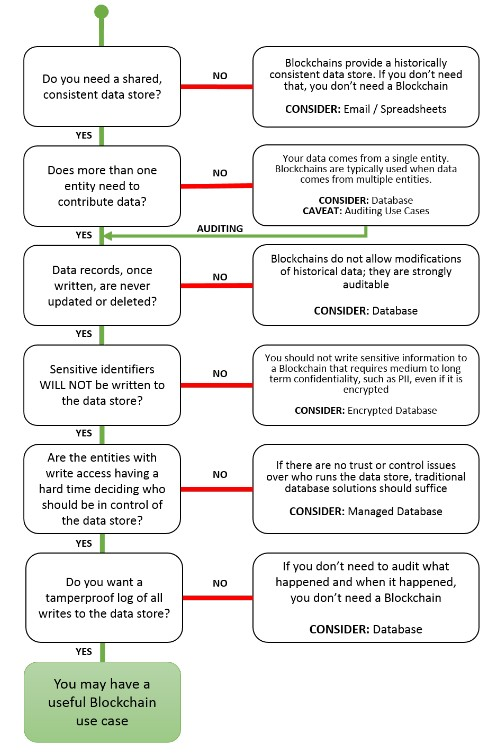
\includegraphics[width=0.7\linewidth]{Figures/Selection_107.jpg}}
    \caption{Diagrama de flujo para determinar un caso de uso Blockchain. De \cite{nist}.}
    \label{fig:use_case_diagram}
\end{figure}

Debido a las confusiones sobre la utilidad de la tecnología Blockchain en una gran cantidad de escenarios, existe una variedad de literatura que describe como determinar un caso de uso Blockchain. Entre otros, el Instituto Nacional de Estándares y Tecnología de Estados Unidos elaboró un diagrama de flujo que ayuda a descartar fácilmente ideas que son mejor implementadas en bases de datos tradicionales.

A continuación se va a analizar el caso de uso planteado con la ayuda de la figura \ref{fig:use_case_diagram} para determinar si la implementación de un sistema de validación de información académica se beneficia de utilizar tecnología Blockchain o no.

\begin{enumerate}
    \item \textbf{¿Se necesita almacenar información de forma compartida y consistente?} Sí, ya que el prototipo apunta a permitir la validación de credenciales académicas por una variedad de entidades, que pueden ser diferentes facultades, Universidades o cualquier otro organismo que necesita determinar que una nota o una historia académica sea válida.
    \item \textbf{¿Es necesario que más que una entidad aporte datos?} Planteando el caso que la UNC reemplaza actas comunes por actas digitales, todas las facultades estarían aportando información. También es posible extender el caso de uso a varias universidades: La validación de credenciales de alumnos que cambian de universidad o quieren realizar un postgrado es facilitada si una multitud de universidades agrega datos.
    \item \textbf{¿No es necesario modificar o eliminar información una vez que fue escrita?} Para el caso del prototipo planteado, la modificación o eliminación de información no es deseada. En su lugar, se desea un historial completo inmutable de lo ocurrido: al revocar un acta, por ejemplo, se mantiene el acta original junto con su acta rectificadora.
    \item \textbf{¿No se va a escribir información sensible o personal en el ledger?} A toda información se va a aplicar un \textit{hash} antes de ser agregada al Blockchain, por ende no se va a escribir nunca información en texto plano.
    \item \textbf{¿Las entidades con acceso de escritura tienen dificultades para decidir quién debe tener el control del almacén de datos?} No existe ningún proyecto para la implementación de un sistema de validación de credenciales académicas centralizado, pero la arquitectura distribuida del Blockchain implica que cada facultad (o en un futuro, Universidad) podría sumarse con pocos recursos y en el momento que sea conveniente.
    \item \textbf{¿Desea un registro inviolable de todas las escrituras en el almacén de datos?} Sí, es crucial que la información sea imposible de alterar.
\end{enumerate}

Luego del análisis efectuado, es posible concluir que el uso de Blockchain para el caso planteado tiene mayores beneficios sobre una base de datos tradicional.

\section{Funcionalidades} \label{sec:funcionalidades}

Luego de la entrevista y de la evaluación del caso de uso, se consideran necesarias las siguientes funcionalidades para el prototipo:

\begin{itemize}
    \item El prototipo debe consistir de un Blockchain con un mínimo de dos organizaciones con dos \textit{peers} cada uno, que comparten información a través de un canal.
    \item Por ende, todos los \textit{peers} deben poder acceder al mismo conjunto de información y el mismo \textit{chaincode}.
    \item El prototipo debe ser capaz que recibir credenciales académicas en texto plano, aplicar una función \textit{hash} a los datos e invocar el \textit{chaincode} correspondiente para que dicha información sea agregada al Blockchain.
    \item Se debe proporcionar la funcionalidad de verificar la existencia de una cierta porción de información: Para validar una nota por ejemplo, se debe poder ingresar la información correspondiente, el prototipo debe aplicar una función \textit{hash} a ella y buscar una coincidencia en el Blockchain para confirmar la validez.
    \item Es necesario proveer la posibilidad de corregir información: Si se requiere revocar un acta, tiene que ser posible agregar su acta rectificativa. Luego el acta original debe ser considerada inválida y ya no debe ser utilizada para validaciones.
\end{itemize}

\section{Definición de los Componentes}

Con el fin de implementar las funcionalidades descritas en la sección \ref{sec:funcionalidades}, en primer lugar se definen los componentes del prototipo en su totalidad.

\begin{enumerate}
    \item \textbf{La red Blockchain: } Se requiere una red de Hyperledger Fabric, compuesta por organizaciones que representan facultades y \textit{peers} que comparten información a través de un canal. El prototipo va a simular tres facultades generando tres organizaciones, cada una con dos \textit{peers}. De esa forma existe redundancia para cada organización: si un \textit{peer} falla, el otro sigue disponible. Además, cada organización tiene que tener una Autoridad de Certificación para otorgar identidades digitales. Va a existir un solo canal al cual las tres organizaciones tienen accesos y por ende un solo \textit{ledger}.
    \item \textbf{La base de datos para el \textit{world state}: } El prototipo a implementar maneja datos a los cuales se aplicó una función de \textit{hash} antes de su almacenamiento. Utilizar el idioma de CouchDB para realizar consultas complejas sobre el estado del \textit{ledger} por ende no es posible. Por eso se eligió LevelDB como la base de datos para almacenar el \textit{world state}.
    \begin{figure}% Example image
        \center{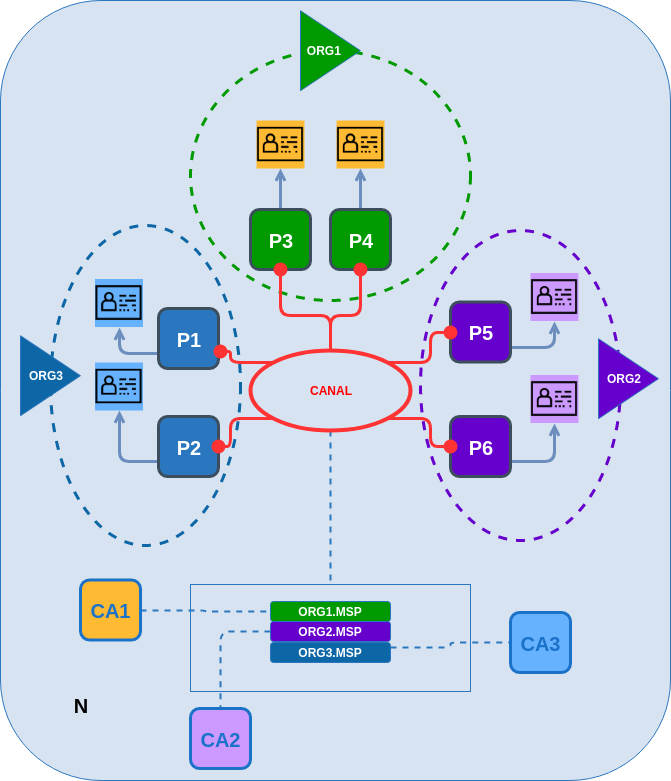
\includegraphics[width=0.8\linewidth]{Figures/network-arquitecture.png}}
        \caption{Diagrama de la red Blockchain a implementar.}
        \label{fig:bc-network}
    \end{figure}
    \item \textbf{El \textit{ordering service}: }Dada la complejidad de configurar Raft o Kafka como servicio de ordenamiento para Hyperledger Fabric se optó por Solo, el servicio de ordenamiento por defecto propuesto para test o pruebas de concepto. Si bien no es recomendado su uso en entornos de producción, cumple con todo lo requerido para el prototipo en cuestión.

    \item \textbf{Elección del lenguaje de programación para el Chaincode: }Las posibilidades para escribir \textit{chaincode} en Hyperledger Fabric son Go, Node.js o Java. Luego de varias pruebas con los 3 lenguajes, la decisión fue tomada a favor de Go: Con Node.js como Java la instanciación del \textit{chaincode} provocaba repetidos errores de tiempo de espera debido a \textit{bugs} en la implementación de Hyperledger Fabric.
    \item \textbf{Elección del SDK: }Hyperledger Fabric provee SDKs en los lenguajes Node.js, Java, Python y Go, dónde los últimos dos todavía no fueron lanzados oficialmente.\cite{hlf_sdks} Para el proyecto se utilizó el SDK en Node.js, ya que la documentación del mismo está muy completa y debido a que el código desarrollado puede ser fácilmente agregado a un \textit{framework} para aplicaciones web.
    \item \textbf{Desarrollo de una API: }El código escrito en Node.js es el código cliente que invoca al \textit{chaincode} a través de los \textit{peers}. Para que sea accesible a través de Internet es necesario el desarrollo de una API REST, que permita llamar las funciones con métodos HTML. La herramienta elegida para esa tarea es Express, un \textit{framework} minimalista y flexible para aplicaciones web y APIs. Está escrito en Javascript, de modo que la integración de las funciones escritas con el SDK se puede realizar sin inconvenientes.
    
    \begin{figure}[H] % Example image
        \center{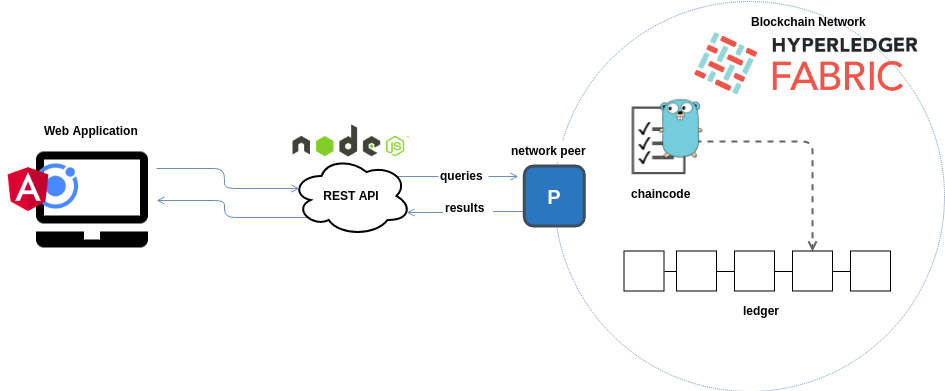
\includegraphics[width=1.0\linewidth]{Figures/arquitecture.png}}
        \caption{Diagrama general de la arquitectura junto con las tecnologías.}
        \label{fig:general_arquitecture}
    \end{figure}
    
    \item \textbf{Desarrollo de una GUI: }La API públicamente expuesta a Internet necesita un \textit{frontend}, o una interfaz web, que acceda a ella. Su funcionalidad consiste en obtener información de la API y mostrarla de forma entendible para el usuario, como también obtener datos ingresados por el usuario y enviarlos para su procesamiento a la API.
    
    Para lograr eso, se decidió utilizar Angular y Ionic: Angular es un \textit{framework} mantenido por Google para el desarrollo de \textit{Single Application Pages (SPAs)}, páginas que adaptan su contenido de forma dinámica a medida que reciben entradas del usuario, en vez de descargar páginas nuevas de un servidor. 
    
    Ionic permite agregar componentes web comúnmente usados a una aplicación escrita en Angular y agiliza así el desarrollo. A su vez viene con librerías como Apache Cordova, que permiten interactuar con dispositivos móviles. De esa forma, una misma aplicación puede ser compilada para un entorno web o un entorno móvil, dependiendo de las necesidades del desarrollador. La figura \ref{fig:ionic_stack} posiciona a Ionic en el contexto de las herramientas para el desarrollo \textit{frontend}.

    \begin{figure}[H]
        \center{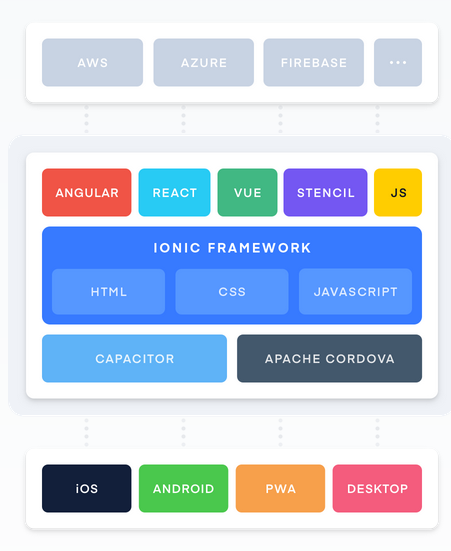
\includegraphics[width=0.6\linewidth]{Figures/Selection_182.png}}
        \caption{El rol de Ionic en el desarrollo \textit{frontend}. De \cite{what-is-ionic}.}
        \label{fig:ionic_stack}
    \end{figure}

\end{enumerate}

\section{Definición de los Requerimientos}
Para especificar el funcionamiento general del sistema, se va a hacer uso del lenguaje de modelado UML. Si bien se trata del desarrollo de un sistema distribuido con una variedad de protocolos y tecnologías, el prototipo final es un producto de \textit{software}, por lo cual un modelado en SysML no se consideró adecuado.

Para poder plantear los requerimientos, primero es necesario definir un diagrama de casos de uso, como se ve en la figura \ref{fig:use_cases}. En el diagrama se puede observar que el objetivo principal es brindar al personal administrativo un sistema de validación de información académica con las funcionalidades de agregar actas, revocarlas y validar la información contenida en las actas cargadas.

\begin{figure}[H]
    \center{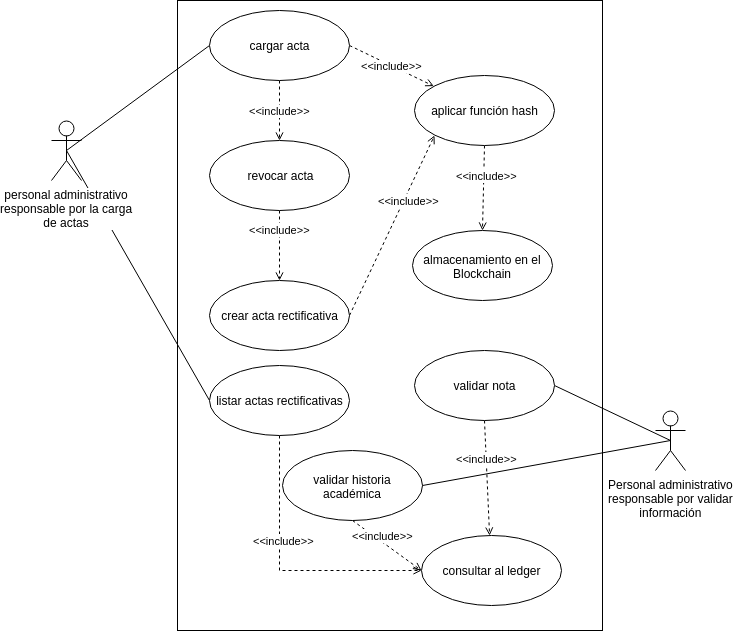
\includegraphics[width=1.0\linewidth]{Figures/use_cases.png}}
    \caption{Diagrama de casos de uso.}
    \label{fig:use_cases}
\end{figure}

Con el diagrama de caso de uso elaborado se pueden definir los siguientes requerimientos de usuario:
\begin{table}[h]
\rowcolors{2}{cyan!20}{cyan!40}
\begin{tabularx}{\textwidth}{|c|X|}
\hline
R-01 & El personal administrativo debe poder cargar la información de un acta nueva al sistema.\\
\hline
R-02 & Para poder verificar la presencia del acta cargada, debe ser posible consultar por el mismo a través de su id.\\
\hline
R-03 & En caso de que se haya cometido un error, debe ser posible revocar el acta y crear su acta rectificativa.\\
\hline
R-04 & Debe ser posible visualizar todas las actas rectificadas.\\
\hline
R-05 & Debe ser posible validar una nota con el sistema: Se debe poder ingresar la información sobre la nota con la nota en texto plano y el sistema debe avisar si la nota se encontró en el sistema o no.\\
\hline
R-06 & Debe ser posible validar la historia académica completa de un alumno de la misma forma que se puede validar una sola nota.\\
\hline
\end{tabularx}
\caption{Requerimientos de usuario.}
\label{table:req_user}
\end{table}

Luego es posible definir los requerimientos funcionales para cada uno de los componentes descritos anteriormente: la red Blockchain, la API y la interfaz gráfica. Se encuentran en los cuadros \ref{table:req_hlf} - \ref{table:req_gui}. Los requerimientos no funcionales se definieron en la tabla \ref{table:req_nofunc}.
\begin{table}[h]
\rowcolors{2}{cyan!20}{cyan!40}
\begin{tabularx}{\textwidth}{|c|X|}
\hline
RF-BC-01 & La red debe ser compuesta por 3 organizaciones y dos \textit{peers} por organización.\\
\hline
RF-BC-02 & La red debe contar con un nodo que provee el servicio de ordenamiento.\\
\hline
RF-BC-03 & Las organizaciones deben contar con una autoridad de certificación cada una para poder agregar usuarios de forma dinámica.\\
\hline
RF-BC-04 & Los \textit{peers} deben ser configurados para poder ejecutar \textit{chaincode} en el lenguaje Golang.\\
\hline
RF-BC-05 & El \textit{chaincode} debe permitir escribir un objeto JSON nuevo en el \textit{ledger}.\\
\hline
RF-BC-06 & El \textit{chaincode} debe permitir recuperar un objeto JSON teniendo la clave.\\
\hline
\end{tabularx}
\caption{Requerimientos funcionales de la red de Hyperledger Fabric.}
\label{table:req_hlf}
\end{table}

\begin{table}
    \rowcolors{2}{cyan!20}{cyan!40}
    \begin{tabularx}{\textwidth}{|c|X|}
    \hline
    RF-API-01 & La API debe proveer un método que permita la subida de un acta. Dicho método debe:
    \begin{itemize}
        \item Recibir un objeto JSON con los datos completos del acta en texto plano.
        \item Aplicar un \textit{hash} a la cabecera del acta y a cada uno de sus renglones.
        \item Formar un objeto JSON que consta del \textit{hash} de la cabecera, el nombre del usuario, un indicador de la validez del acta como el conjunto de todos los renglones del acta en formato \textit{hash}.
        \item Invocar el \textit{chaincode} mencionado en RF-BC-06 que permita escribir dicho objeto en el Blockchain.
    \end{itemize}\\
    \hline
    RF-API-02 & La API debe proveer un método que permita recuperar el acta como fue escrito en el Blockchain, haciendo uso del \textit{chaincode} descrito en el requerimiento RF-BC-06.\\
    \hline
    RF-API-03 & La API debe contar con un método que permita revocar a un acta. Para eso debe
    \begin{itemize}
        \item Verificar que el acta realmente puede ser rectificada.
        \item Marcar el acta a revocar como inválida.
        \item Generar un acta nueva con los renglones corregidos.
    \end{itemize}\\
    \hline
    RF-API-04 & La API debe proveer una función que permita indicar la validez o invalidez de una nota. Para cumplir con esa funcionalidad, debe
    \begin{itemize}
        \item Recibir el id del acta en texto plano como también la información de la nota que se encuentra en el renglón correspondiente del acta.
        \item Luego debe aplicar la función \textit{hash} al renglón y buscar el acta indicada en el Blockchain.
        \item Por último debe verificar si existe una coincidencia entre uno de los renglones recuperados y el calculado.
    \end{itemize}\\
    \hline
    RF-API-05 & La API debe poder indicar si una historia académica es válida o no, recibiendo la información necesaria y procediendo igual que en los pasos del requerimiento RF-API-04.\\
    \hline
    RF-API-06 & La API debe notificar cualquier tipo de error: En el caso que un acta no fue encontrado o en el caso de un problema de conexión o autenticación con el Blockchain.\\
    \hline
\end{tabularx}
\caption{Requerimientos funcionales de la API.}
\label{table:req_api}
\end{table}

\begin{table}[h]
    \rowcolors{2}{cyan!20}{cyan!40}
    \begin{tabularx}{\textwidth}{|c|X|}
    \hline
    RF-GUI-01 & La GUI debe contar con una página que permite la selección y ejecución de las siguientes tareas:
    \begin{enumerate}
        \item Cargar un acta nueva al sistema.
        \item Buscar un acta con su id.
        \item Validar una nota.
        \item Validar una historia académica.
        \item Revocar un acta.
        \item Consultar todos los actas rectificadas.
    \end{enumerate}\\
    \hline
    RF-GUI-02 & Para poder cumplir con cada tarea, la GUI debe proveer campos que permitan al usuario ingresar los datos necesarios para efectuar la tarea.\\
    \hline
    RF-GUI-03 & La GUI debe estar en los idiomas inglés y español. \\
    \hline
    RF-GUI-04 & Durante el tiempo de ejecución de consultas o escrituras en el Blockchain, la GUI debe indicar esto mismo al usuario.\\
    \hline
    RF-GUI-05 & La GUI debe notificar el éxito o fracaso de cada operación debidamente al usuario.\\
    \hline
    \end{tabularx}
    \caption{Requerimientos funcionales de la interfaz gráfica de usuario. (\textit{Graphical User Interface})}
    \label{table:req_gui}
\end{table}

\begin{table}[h]
    \rowcolors{2}{cyan!20}{cyan!40}
    \begin{tabularx}{\textwidth}{|c|X|}
    \hline
    RNF-01 & El sistema debe contar con pruebas y tests integrales de los seis requerimientos de usuario.\\
    \hline
    RNF-02 & El código del \textit{chaincode} debe estar escrito en el lenguaje Golang, la API debe desarrollarse en Node.js y para la Interfaz Gráfica se debe usar Typescript.\\
    \hline
    RNF-03 & La GUI debe indicar éxito o fracaso de una operación en un tiempo no mayor a los diez segundos.\\
    \hline
    RNF-04 & La GUI debe contar con un instructivo para que un usuario sin conocimiento previo puede aprender a utilizar el sistema.\\
    \hline
    \end{tabularx}
    \caption{Requerimientos no funcionales del sistema.}
    \label{table:req_nofunc}
\end{table}

Para poder comprender mejor cúal es la relación estructural entre las diferentes tecnologías empleados en el prototipo, se ofrece un diagrama de componentes, realizado en la figura \ref{fig:components}. Se distinguen 3 componentes principales: El \textit{frontend}, la aplicación y la red de Hyperledger Fabric. La aplicación se divide en el código funcional de la aplicación en sí, que convierte, por ejemplo, las actas en texto plano a un \textit{hash}, y el SDK de Hyperledger Fabric que brinda las librerías necesarias para invocar \textit{chaincode} en los diferentes \textit{peers} a través de una interfaz \textit{shim}.

\begin{figure}[H]
    \center{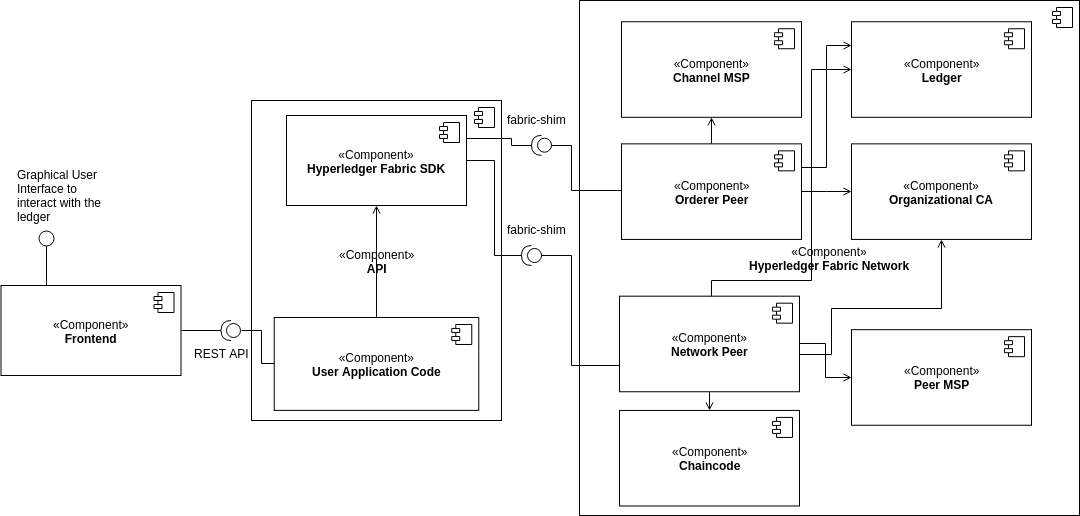
\includegraphics[width=1.0\linewidth]{Figures/components.png}}
    \caption{Diagrama de componentes.}
    \label{fig:components}
\end{figure}


\section{Definición del Comportamiento}
Para poder entender cómo interactúan los componentes diagramados, se emplearon dos diagramas de secuencia. El primero, la figura \ref{fig:secuencia1}, muestra el flujo de mensajes en el caso de una lectura del \textit{ledger}, por ejemplo para verificar la validez de un acta. En el diagrama se puede observar lo que ya se describió en la sección \ref{sec:aplicaciones_y_redBC}: Para realizar una lectura, es necesario interactuar con un solo \textit{peer} de la red. Éste puede ejecutar el \textit{chaincode} sobre su copia del \textit{ledger} local y proveer resultados sin tener que involucrar otros participantes.

\begin{figure}
    \center{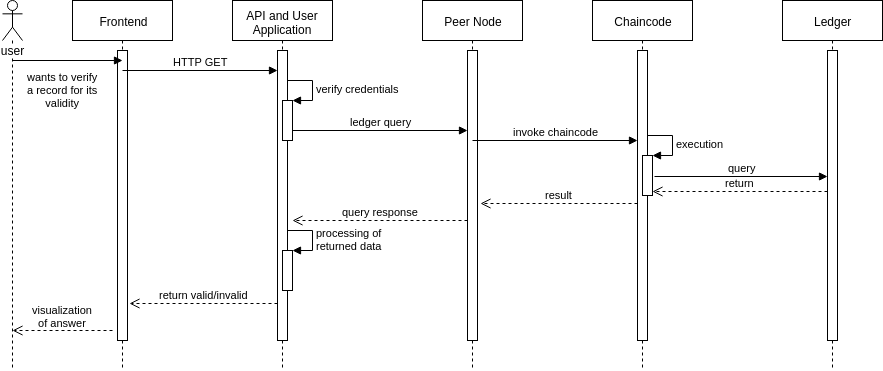
\includegraphics[width=1.0\linewidth]{Figures/sequence1.png}}
    \caption{Diagrama de secuencia para lecturas del \textit{ledger}.}
    \label{fig:secuencia1}
\end{figure}

En la figura \ref{fig:secuencia2} se puede observar el diagrama de secuencia para caso de escritura del \textit{leger}: La aplicación envía una propuesta de aprobación de la transacción (\textit{endorsement proposal}) a una cantidad definida de \textit{peers}. En el diagrama se ve que la propuesta se envía a tres \textit{peers}, pero pueden ser más o menos según la política de aprobación establecida por las organizaciones. Cada \textit{peer} ejecuta el \textit{chaincode} correspondiente y retorna los resultados a la aplicación, cuya obligación es verificar que coinciden. Luego, esta envía un mensaje con todas las respuestas al servicio que ordena las transacciones. Cuando un bloque nuevo es creado, las transacciones en cuestión van a estar incluidas en él y todos los \textit{peers} controlan que se encuentran válidas y que se respetaron las políticas de aprobación. Una vez que terminaron, un \textit{peer} notifica la aplicación para que el usuario pueda saber si la escritura en el Blockchain fue exitosa o no.

\begin{figure}[H]
    \center{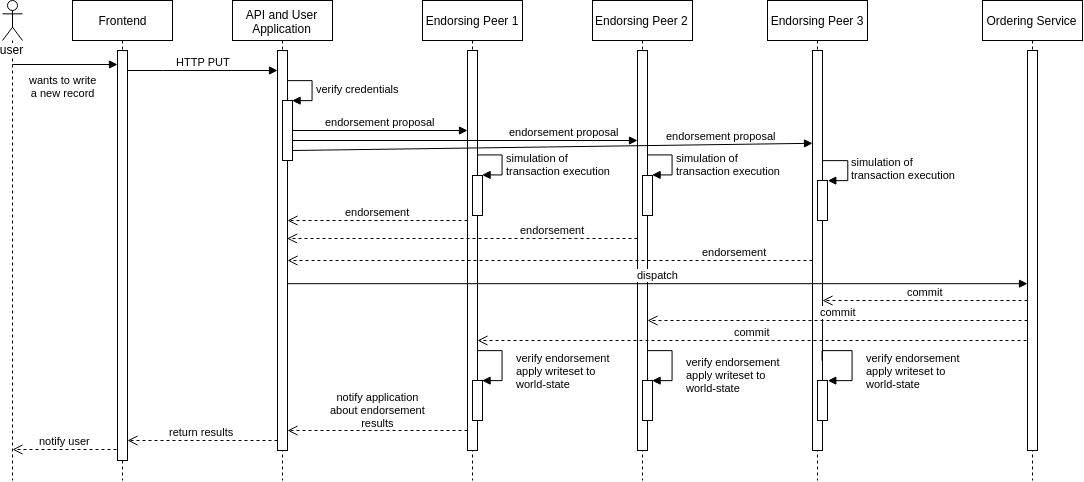
\includegraphics[width=1.0\linewidth]{Figures/sequence-write.png}}
    \caption{Diagrama de secuencia para escrituras del \textit{ledger}.}
    \label{fig:secuencia2}
\end{figure}

\section{Riesgos}
La evaluación de riesgos de un proyecto busca posibles eventos no deseados que pueden perjudicar o amenazar al proyecto con el objetivo de minimizarlos o, en el caso de que ocurran, controlar su impacto sobre el proyecto.

El objetivo de la presente sección es establecer criterios, identificar posibles riesgos, asignar prioridades a los mismos, evaluar su probabilidad y encontrar estrategias que permiten resolver los mismos o minimizar sus efectos.

\subsection{Criterios}
Los riesgos se clasifican según dos criterios: su probabilidad y la gravedad en el caso de su ocurrencia. A continuación figuran las siguientes probabilidades y gravedades que se tuvieron en cuenta según \cite{sommerville}:

\begin{enumerate}
    \item Riesgo muy bajo (\textless10\%)
    \item Riesgo bajo (10 - 25\%)
    \item Riesgo moderado (25 - 50\%)
    \item Riesgo alto (50 - 75\%)
    \item Riesgo muy alto (\textgreater75\%)
\end{enumerate}

\begin{enumerate}
    \item Efectos insignificantes
    \item Efectos tolerables
    \item Efectos graves
    \item Efectos catastróficos
\end{enumerate}

La combinación de ambos criterios permite priorizar los riesgos teniendo en cuenta ambos factores.
\begin{table}[h]
    \begin{tabular}{|c|c|c|c|c|}
    \hline
    \textbf{Probabilidad/Efecto}& \textbf{Insignificante} & \textbf{Tolerable} & \textbf{Grave} & \textbf{Catastrófico}\\
    \hline
    \textbf{Muy baja} &\cellcolor{YellowGreen} &\cellcolor{YellowGreen} &\cellcolor{YellowGreen} & \cellcolor{yellow}\\
    \hline
    \textbf{Baja} & \cellcolor{YellowGreen} & \cellcolor{YellowGreen} & \cellcolor{yellow} & \cellcolor{yellow}\\
    \hline
    \textbf{Moderada} & \cellcolor{YellowGreen} & \cellcolor{yellow} &\cellcolor{yellow} & \cellcolor{red}\\
    \hline
    \textbf{Alta} & \cellcolor{yellow} & \cellcolor{yellow} & \cellcolor{red} & \cellcolor{red} \\
    \hline
    \textbf{Muy alta} &\cellcolor{yellow} & \cellcolor{red}& \cellcolor{red}&\cellcolor{red}\\
    \hline
    \end{tabular}
    \caption{Probabilidad de riesgos vs. su efecto}
\end{table}
En base a la combinación realizada, se consideran los riesgos que se encuentran dentro del área verde como riesgos de menor prioridad, los riesgos en el área amarilla como riesgos de prioridad intermedia y los riesgos en el área roja como riesgos de prioridad alta.
\subsection{Identificación de Riesgos}
En la primera etapa de la gestión de riesgos, se buscan los posibles riesgos relacionados al proyecto, distinguiendo las 5 categorías siguientes:
\begin{itemize}
    \item \textbf{Riesgos de tecnología:} Riesgos relacionados a hardware o \textit{software} con el que se está desarrollando el proyecto.
    \item \textbf{Riesgos personales:} Relacionados con el personal en el equipo de desarrollo.
    \item \textbf{Riesgos de requerimientos:} Surgen de modificaciones de los requerimientos.
    \item \textbf{Riesgos de estimación:} relacionados a la estimación de recursos requeridos para el desarrollo del proyecto.
\end{itemize}
Los riesgos que se identificaron para el presente proyecto integrador figuran en la tabla \ref{identification_risks}.
\begin{table}[h]
    \begin{tabular}{|m{2cm}|m{7.5cm}|m{3.5cm}|}
    \hline
    \textbf{Código} & \textbf{Descripción} & \textbf{Tipo de riesgo}\\
    \hline
    Riesgo-01 & Problemas de funcionamiento o avería de la PC de desarrollo durante el tiempo de desenvolvimiento. & Tecnológico\\
    \hline
    Riesgo-02 & Incompatibilidad de versiones o librerías instaladas en la máquina de desarrollo con los \textit{frameworks} usados. & Tecnológico \\
    \hline
    Riesgo-03 & Funcionalidades sin implementar en el \textit{framework} de Hyperledger Fabric. & Requerimientos\\
    \hline
    Riesgo-04 & Demoras durante el desarrollo del proyecto debido a trabajo u otros inconvenientes personales. & Personales y Estimación \\
    \hline
    Riesgo-05 & Abandono del proyecto. & Personal \\
    \hline
    Riesgo-06 & Errores en la implementación de los \textit{frameworks} elegidos. & Tecnológico, Requerimientos y Estimación\\
    \hline
    Riesgo-07 & Falta de conocimiento para el uso de los \textit{frameworks}, del \textit{software} o los lenguajes de programación elegidos. & Estimación \\
    \hline
    Riesgo-08 & Falta de documentación o soporte de los \textit{frameworks} elegidos. & Estimación \\
    \hline
    Riesgo-09 & Rechazo de la implementación por parte del usuario, debido a desconfianza que genera una nueva tecnología. & Estimación \\
    \hline 
    \end{tabular}
    \caption{Riesgos identificados para el proyecto}
\label{identification_risks}
\end{table}

\subsection{Análisis de Riesgos}
\newcolumntype{C}[1]{>{\centering\arraybackslash}m{#1}}
En el cuadro \ref{analisys_risks} se ordenaron los riesgos según su importancia luego de estimar probabilidad e indicar el efecto.
\begin{table}
    \begin{tabular}{|C{2cm}|m{3.5cm}|C{2.4cm}|C{2.5cm}|C{2.4cm}|}
    \hline
    \textbf{Código} & \textbf{Riesgo} & \textbf{Probabilidad} & \textbf{Efecto} & \textbf{Importancia}\\
    \hline
    Riesgo-02 & Incompatibilidad de versiones o librerías instaladas en la máquina de desarrollo con los \textit{frameworks} usados. & Moderada & Insignificante &\cellcolor{YellowGreen} Prioridad baja\\
    \hline
    Riesgo-01 & Problemas de funcionamiento o avería de la PC de desarrollo durante el tiempo de desenvolvimiento. & Baja & Grave & \cellcolor{yellow} Prioridad Intermedia\\
    \hline
    Riesgo-03 & Funcionalidades sin implementar en el \textit{framework} de Hyperledger Fabric. & Alta & Tolerable & \cellcolor{yellow}Prioridad Intermedia\\
    \hline
    Riesgo-05 & Abandono del proyecto. & Muy baja & Catastrófico & \cellcolor{yellow}Prioridad Intermedia\\
    \hline
    Riesgo-06 & Errores en la implementación de los \textit{frameworks} elegidos. & Alta & Tolerable & \cellcolor{yellow} Prioridad intermedia\\
    \hline
    Riesgo-07 & Falta de conocimiento para el uso de los \textit{frameworks}, del \textit{software} o los lenguajes de programación elegidos. & Alta & Tolerable &\cellcolor{yellow} Prioridad intermedia\\
    \hline
    Riesgo-08 & Falta de documentación o soporte de los \textit{frameworks} elegidos. & Moderada & Grave &\cellcolor{yellow} Prioridad intermedia \\
    \hline   
    Riesgo-04 & Demoras durante el desarrollo del proyecto debido a trabajo u otros inconvenientes personales. & Alta & Grave & \cellcolor{red}Prioridad alta\\
    \hline
    Riesgo-09 & Rechazo de la implementación por parte del usuario, debido a desconfianza que genera una nueva tecnología. & Alta & Grave & \cellcolor{red}Prioridad alta\\
    \hline
    \end{tabular}
    \caption{Riesgos clasificados según su probabilidad y efecto.}
\label{analisys_risks}
\end{table}
\subsection{Planificación de Riesgos}
En la presente sección se describen las estrategias para manejar cada riesgo identificado. Los cuadros \ref{risk-strategy1} y \ref{risk-strategy2} detallan los pasos a seguir en el caso de la ocurrencia de cualquier riesgo.
\begin{table}[h]
    \begin{tabular}{|C{2cm}|m{3.5cm}|C{8cm}|}
    \hline
    \textbf{Código} & \textbf{Riesgo} & \textbf{Estrategias de Manejo del riesgo}\\
    \hline
    Riesgo-01 & Problemas de funcionamiento o avería de la PC de desarrollo durante el tiempo de desenvolvimiento. & \begin{itemize}
        \item Implementación de una estrategia de respaldo de información en la nube con repositorios de Gitlab.
        \item Realización de la operación \textit{push} al repositorio una o más veces por día.
        \item Arreglo o reemplazo de la máquina de desarrollo en el caso de una avería.
    \end{itemize}\\
    \hline
    Riesgo-02 & Incompatibilidad de versiones o librerías instaladas en la máquina de desarrollo con los \textit{frameworks}  usados. & \begin{itemize}
        \item Lectura cuidadosa de tutoriales de instalación y prerequisitos.
        \item Uso de Docker para ganar mayor flexibilidad con versiones de librerías o lenguajes de programación.
    \end{itemize}\\
    \hline
    Riesgo-03 & Funcionalidades sin implementar en el framework de Hyperledger Fabric. & Adaptación de los requerimientos a las posibilidades del \textit{framework}.\\
    \hline
    Riesgo-04 & Demoras durante el desarrollo del proyecto debido a trabajo u otros inconvenientes personales. & \begin{itemize}
        \item Comunicación fluida con director y codirector del trabajo.
        \item Reducción de obligaciones laborales y extracurriculares a lo mínimo e indispensable.
    \end{itemize}\\
    \hline
    Riesgo-05 & Abandono del proyecto &
    \begin{itemize}
        \item Comunicación fluida con director y codirector del trabajo.
        \item Definición clara del alcance del proyecto para minimizar las posibilidades de desborde en términos de tiempo y trabajo.
    \end{itemize}\\
    \hline
\end{tabular}
\caption{Estrategias de manejo de riesgos parte uno}
\label{risk-strategy1}
\end{table}

\begin{table}[h]
    \begin{tabular}{|C{2cm}|m{3.5cm}|C{8cm}|}
    \hline
    Riesgo-06 & Errores en la implementación de los \textit{frameworks} elegidos. &
    \begin{itemize}
        \item Implementación de \textit{workarounds} descritos en la documentación o páginas de seguimientos de \textit{issues} como Jira.
        \item Modificación de la implementación para poder cumplir con el requerimiento.
        \item Adaptación del requerimiento.
    \end{itemize}\\
    \hline
    Riesgo-07 & Falta de conocimiento para el uso de los \textit{frameworks}, del \textit{software} o los lenguajes de programación elegidos. & \begin{itemize}
        \item Lectura de tutoriales y realización de cursos de tiempo corto para lograr una introducción en temas cuyo desconocimiento impide el avance del proyecto.
        \item Empleo y modificación de ejemplos previstos para el aprendizaje.
        \item Consultas a programadores experimentados en los campos en cuestión.
     \end{itemize}\\
     \hline
     Riesgo-08 & Falta de documentación o soporte de los \textit{frameworks} elegidos. & \begin{itemize}
        \item Búsqueda de explicaciones adicionales en foros de usuarios como Stackoverflow.
        \item Consultas en canales de chat de desarrolladores como Slack o Rocketchat.
        \item Modificación de la implementación para poder cumplir con el requerimiento.
        \item Adaptación del requerimiento.
     \end{itemize}\\
     \hline
     Riesgo-09 & Rechazo de la implementación por parte del usuario, debido a desconfianza que genera una nueva tecnología. & \begin{itemize}
        \item Explicación de la tecnología y capacitación del personal.
        \item Prueba de piloto para identificar mejoras en cuanto a la usabilidad.
     \end{itemize}\\
     \hline
    \end{tabular}
    \caption{Estrategias de manejo de riesgos parte dos}
    \label{risk-strategy2}
\end{table}

\section{Control de Versiones}
Para el control de versiones, se utilizó un repositorio de Gitlab disponible bajo la URL \url{https://gitlab.com/ELeonhardt/final-project-codebase}

Si bien Git es una herramienta para para mejorar la colaboración entre varios programadores, también se justifica su uso cuando una sola persona está desarrollando el proyecto. Usar un repositorio permite tener acceso remoto al proyecto desde cualquier equipo, teniendo así una copia de seguridad del proyecto completo en la nube. A su vez, se mantiene un historial de versiones y en caso de ser necesario, es posible volver a una versión anterior o comparar las diferencias entre dos versiones distintas.

\newpage
